%BEGIN TICKET 47
\begin{definition}
    Длина пути $l(\gamma) = \sup \sum\limits_{k=1}^n \rho(\gamma(t_k), \gamma(t_{k-1}))$, где  $t_k$ --- дробление отрезка.
    \begin{figure}[h!]
        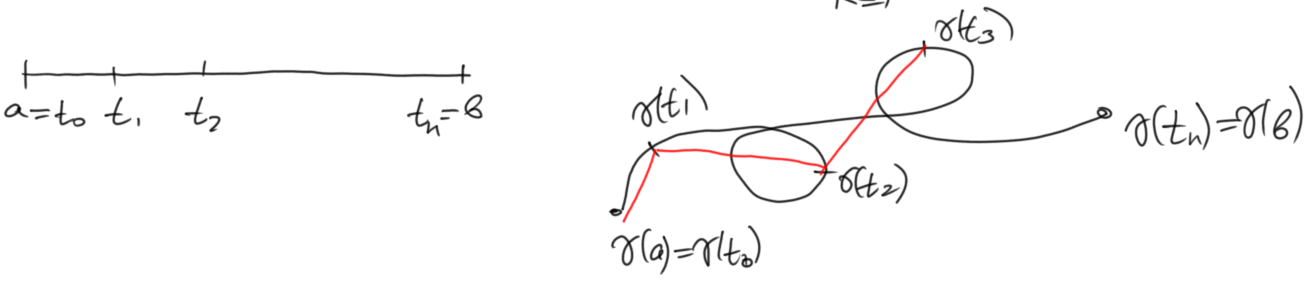
\includegraphics[width=\textwidth]{curve_length}
    \end{figure}
\end{definition}
\begin{remark}
    Длины эквивалентных путей равны.
\end{remark}
\begin{properties}
    \begin{enumerate}
        \item $l(\gamma) \ge \rho(\gamma(a), \gamma(b))$. Можно просто взять дробление состоящее из двух точек.
        \item $l(\gamma) \ge$ длина вписанной в нее ломаной.
    \end{enumerate}
\end{properties}
\begin{theorem}
    Пусть есть $\gamma\!: [a, b] \to X$.  $c \in [a, b]$. 

    $l(\gamma) = l(\gamma \Big|_{[a, c]}) + l(\gamma \Big|_{[c, b]})$.

    Обозначим куски за  $\gamma_1, \gamma_2$.
\end{theorem}
\begin{proof}
    Нам нужно доказать какое-то равенство, поэтому докажем два неравенства!
    \begin{itemize}
        \item $\ge$. Давайте вписывать ломанные. Впишем какую-то ломанную в $\gamma_1$ и еще какую-то в $\gamma_2$. Пусть получились дробления $a = t_0 < t_1 < t_2 < \ldots < t_n = u_0 < \ldots < u_m = b$ --- получилось дробление $[a, b]$.

            Тогда посчитаем сумму:  $\sum\limits_{k=1}^n \rho(\gamma(t_{k-1}), \gamma(t_k)) + \sum\limits_{k=1}^n \rho(\gamma(u_{k-1}), \gamma(u_k)) \le l(\gamma)$. Заменим первое слагаемое на $\sup$: $\sup \ldots + \sum\limits_{k=1}^n \rho(\gamma(u_{k-1}), u_k) \le l(\gamma)$. А этот $\sup$ --- длина  $\gamma_1$. Встает вопрос почему можно переходить. Мы знаем, что все числа меньше, то и супремум меньше, поэтому переход корректный. Дальше заменяем правый $\sup$. В итоге получаем  $l(\gamma_1) + l(\gamma_2) \le l(\gamma)$.
        \item Возьмем дробление $\gamma$  $t_i$. Посмотрим на сумму  $S = \sum\limits_{j=1}^n\rho(\gamma(t_{j-1}), \gamma(t_j))$. 

            Возьмем дробление $t_i$ и добавим в него точку  $c$. Получаем: 
             \begin{align*}
                S \le \sum_{j=1}^k \rho(\gamma(t_{j-1}), \gamma(t_j)) + \rho(\gamma(t_k), \gamma(c)) + \rho(\gamma(c), \gamma(t_{k+1})) + \sum_{j = k + 2}^n \rho(\gamma(t_{j-1}), \gamma(t_j))
            \end{align*}
            
            А теперь увидим, что первые два слагаемых $\le l(\gamma_1)$, а вторые два $\le l(\gamma_2)$.
    \end{itemize}
\end{proof}
%END TICKET 47